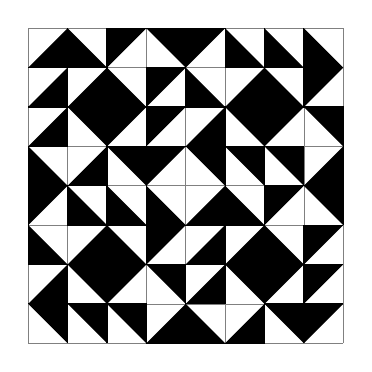
\begin{tikzpicture}[scale=0.5]
 \draw [step=1cm,gray,very thin](0,-1) grid (8,7); 
 \draw[opacity=1,fill=black](0,0)--(1,0)--(1,-1); 
 \draw[opacity=1,fill=black](1,1)--(1,0)--(0,0); 
 \draw[opacity=1,fill=black](1,1)--(0,1)--(0,2); 
 \draw[opacity=1,fill=black](0,2)--(0,3)--(1,3); 
 \draw[opacity=1,fill=black](1,3)--(0,3)--(0,4); 
 \draw[opacity=1,fill=black](1,5)--(1,4)--(0,4); 
 \draw[opacity=1,fill=black](1,6)--(1,5)--(0,5); 
 \draw[opacity=1,fill=black](1,7)--(1,6)--(0,6); 
 \draw[opacity=1,fill=black](1,0)--(2,0)--(2,-1); 
 \draw[opacity=1,fill=black](1,1)--(2,1)--(2,0); 
 \draw[opacity=1,fill=black](2,2)--(2,1)--(1,1); 
 \draw[opacity=1,fill=black](2,2)--(1,2)--(1,3); 
 \draw[opacity=1,fill=black](2,4)--(2,3)--(1,3); 
 \draw[opacity=1,fill=black](1,5)--(2,5)--(2,4); 
 \draw[opacity=1,fill=black](2,6)--(2,5)--(1,5); 
 \draw[opacity=1,fill=black](2,6)--(1,6)--(1,7); 
 \draw[opacity=1,fill=black](2,0)--(3,0)--(3,-1); 
 \draw[opacity=1,fill=black](2,0)--(2,1)--(3,1); 
 \draw[opacity=1,fill=black](3,1)--(2,1)--(2,2); 
 \draw[opacity=1,fill=black](3,2)--(2,2)--(2,3); 
 \draw[opacity=1,fill=black](2,4)--(3,4)--(3,3); 
 \draw[opacity=1,fill=black](2,4)--(2,5)--(3,5); 
 \draw[opacity=1,fill=black](3,5)--(2,5)--(2,6); 
 \draw[opacity=1,fill=black](2,6)--(2,7)--(3,7); 
 \draw[opacity=1,fill=black](4,0)--(4,-1)--(3,-1); 
 \draw[opacity=1,fill=black](3,1)--(4,1)--(4,0); 
 \draw[opacity=1,fill=black](3,1)--(3,2)--(4,2); 
 \draw[opacity=1,fill=black](4,2)--(3,2)--(3,3); 
 \draw[opacity=1,fill=black](3,3)--(3,4)--(4,4); 
 \draw[opacity=1,fill=black](3,4)--(3,5)--(4,5); 
 \draw[opacity=1,fill=black](3,5)--(3,6)--(4,6); 
 \draw[opacity=1,fill=black](3,7)--(4,7)--(4,6); 
 \draw[opacity=1,fill=black](5,-1)--(4,-1)--(4,0); 
 \draw[opacity=1,fill=black](5,1)--(5,0)--(4,0); 
 \draw[opacity=1,fill=black](5,2)--(5,1)--(4,1); 
 \draw[opacity=1,fill=black](5,3)--(5,2)--(4,2); 
 \draw[opacity=1,fill=black](4,4)--(5,4)--(5,3); 
 \draw[opacity=1,fill=black](5,5)--(5,4)--(4,4); 
 \draw[opacity=1,fill=black](5,5)--(4,5)--(4,6); 
 \draw[opacity=1,fill=black](4,6)--(4,7)--(5,7); 
 \draw[opacity=1,fill=black](6,0)--(6,-1)--(5,-1); 
 \draw[opacity=1,fill=black](5,1)--(6,1)--(6,0); 
 \draw[opacity=1,fill=black](6,2)--(6,1)--(5,1); 
 \draw[opacity=1,fill=black](6,2)--(5,2)--(5,3); 
 \draw[opacity=1,fill=black](5,4)--(6,4)--(6,3); 
 \draw[opacity=1,fill=black](5,5)--(6,5)--(6,4); 
 \draw[opacity=1,fill=black](6,6)--(6,5)--(5,5); 
 \draw[opacity=1,fill=black](6,6)--(5,6)--(5,7); 
 \draw[opacity=1,fill=black](6,0)--(7,0)--(7,-1); 
 \draw[opacity=1,fill=black](6,0)--(6,1)--(7,1); 
 \draw[opacity=1,fill=black](7,1)--(6,1)--(6,2); 
 \draw[opacity=1,fill=black](6,2)--(6,3)--(7,3); 
 \draw[opacity=1,fill=black](6,4)--(7,4)--(7,3); 
 \draw[opacity=1,fill=black](6,4)--(6,5)--(7,5); 
 \draw[opacity=1,fill=black](7,5)--(6,5)--(6,6); 
 \draw[opacity=1,fill=black](7,6)--(6,6)--(6,7); 
 \draw[opacity=1,fill=black](7,-1)--(7,0)--(8,0); 
 \draw[opacity=1,fill=black](7,0)--(7,1)--(8,1); 
 \draw[opacity=1,fill=black](7,1)--(7,2)--(8,2); 
 \draw[opacity=1,fill=black](7,3)--(8,3)--(8,2); 
 \draw[opacity=1,fill=black](8,4)--(8,3)--(7,3); 
 \draw[opacity=1,fill=black](7,5)--(8,5)--(8,4); 
 \draw[opacity=1,fill=black](7,5)--(7,6)--(8,6); 
 \draw[opacity=1,fill=black](8,6)--(7,6)--(7,7); 
\end{tikzpicture} 